\section{Metodologia}\label{sec:metodologia}

Esta seção detalha a metodologia desenvolvida para a análise otimizada e o projeto paramétrico de pontes de madeira roliça. Para a consecução deste objetivo, construiu-se uma plataforma computacional dedicada à definição automatizada das dimensões estruturais, especificamente das longarinas e das pranchas do tabuleiro.

O ambiente computacional foi integralmente desenvolvido em linguagem \textit{Python}, adotando uma arquitetura cliente-servidor flexível, com interface web construída por meio da biblioteca \textit{Streamlit} e disponibilizada em acesso livre \parencite{ReliaBridge2026}. Internamente, o motor de simulação e busca evolutiva integra pacotes avançados de programação científica. A otimização multiobjetivo baseada em metaheurísticas é conduzida por algoritmos genéticos da biblioteca \texttt{pymoo} \parencite{blank2020}, enquanto a quantificação de incertezas e a análise de sensibilidade global estocástica são processadas pela biblioteca \texttt{UQpy} \parencite{Olivier2020}.

A plataforma permite uma transição fluida entre o dimensionamento paramétrico tradicional e a concepção orientada por otimização de Pareto. Após o processamento algorítmico do modelo da ponte, o usuário obtém acesso integral ao memorial de cálculo gerado pela ferramenta. Esse relatório detalha o desempenho da estrutura frente aos esforços solicitantes e aos deslocamentos normativos, fornecendo o escrutínio completo das verificações de segurança e de serviço, com a indicação exata dos critérios em que a configuração da ponte obteve êxito ou falhou.

O fluxo metodológico consolidado, ilustrado na Figura~\ref{fig:fluxograma}, é composto pelas seguintes etapas: (i) definição da geometria e das cargas permanentes; (ii) definição do trem tipo; (iii) cálculo estrutural dos esforços solicitantes e deslocamentos; (iv) combinação de ações nos estados limites último e de serviço; (v) determinação das resistências de projeto e avaliação de propriedades segundo a NBR 7190; (vi) otimização estocástica via NSGA-II; (vii) análise de sensibilidade global de Sobol; e (viii) obtenção do conjunto de soluções viáveis da fronteira eficiente.

\begin{figure}[!ht]
\centering
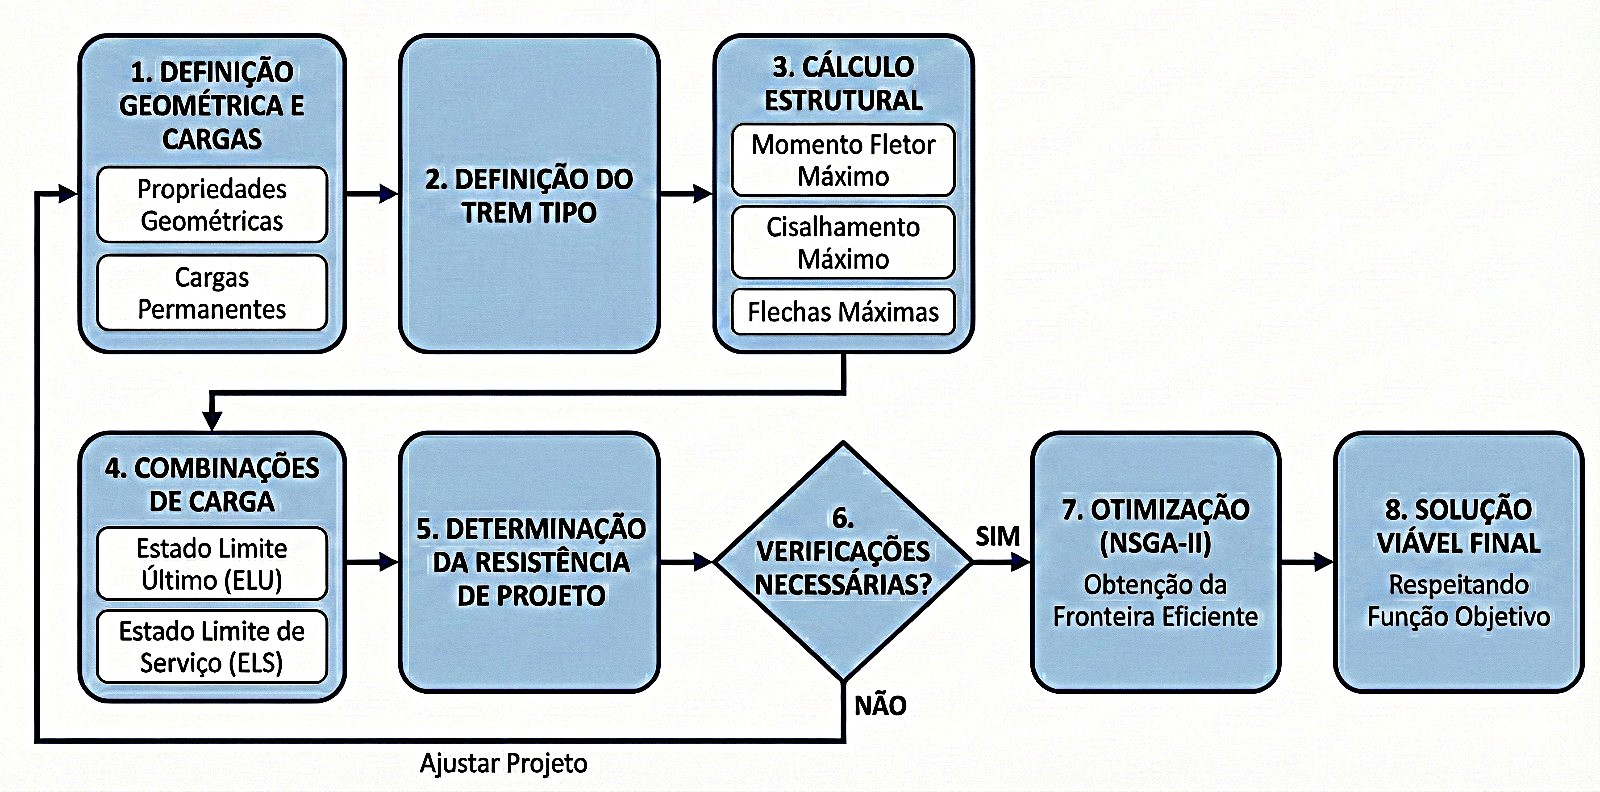
\includegraphics[width=0.9\textwidth]{figuras/fluxograma.jpeg}
\caption{Fluxograma da otimização e análise do dimensionamento de pontes de madeira.}
\label{fig:fluxograma}
\end{figure}

\subsection{Definição do modelo de teste e propriedades dos materiais}\label{sec:modelo_teste}

Para testar a ferramenta e demonstrar a aplicação direta do algoritmo implementado, adotou-se como objeto de estudo a ponte de estrada vicinal de pista simples, dimensionada para suportar o tráfego do trem tipo TB-240 estipulado pela ABNT NBR 7188 \parencite{nbr7188}. Essa configuração é representativa de acessos rurais e vias locais, nas quais a demanda por projetos econômicos e duráveis em madeira é proeminente. Em vez de um único caso isolado, o trabalho explora uma matriz de configurações que combina quatro vãos teóricos com as cinco classes de resistência normativas, conforme detalhado na Seção~\ref{sec:casos}, de modo a permitir a leitura do efeito isolado de cada fator.

A modelagem mecânica dos elementos estruturais acompanha rigorosamente as prescrições normativas brasileiras. As variações de características do material e a definição das propriedades adotadas nas simulações foram estabelecidas em conformidade com a ABNT NBR 7190-3:2022. As propriedades elásticas e as classes de resistência de base para espécies de florestas nativas (D20 a D60), derivadas de ensaios em corpos de prova isentos de defeitos, estão dispostas na Tabela~\ref{tab:classes_madeira}.

Ressalta-se que, para a madeira pertencente ao grupo das dicotiledôneas, a norma técnica define a relação direta entre a resistência característica à compressão paralela às fibras ($f_{c0,k}$) e a resistência característica à flexão ($f_{m,k}$) pela razão $f_{c0,k} / f_{m,k} = 0{,}77$. Logo, os valores de resistência à flexão empregados pela plataforma para a formulação das restrições de estado limite foram deduzidos analiticamente a partir dessa premissa.

\begin{table}[!ht]
\caption{Classes de resistência de espécies de florestas nativas e resistência à flexão calculada.\label{tab:classes_madeira}}
\begin{threeparttable}
\begin{tabular*}{\columnwidth}{@{\extracolsep{\fill}}lccccc@{\extracolsep{\fill}}}
\toprule
Classes & $f_{c0,k}$ (MPa) & $f_{m,k}$ (MPa) & $f_{v0,k}$ (MPa) & $E_{c0,med}$ (MPa) & Densidade a 12\% (kg/m\textsuperscript{3}) \\
\midrule
D20 & 20 & 26,0 & 4 & 10 000 & 500 \\
D30 & 30 & 39,0 & 5 & 12 000 & 625 \\
D40 & 40 & 51,9 & 6 & 14 500 & 750 \\
D50 & 50 & 64,9 & 7 & 16 500 & 850 \\
D60 & 60 & 77,9 & 8 & 19 500 & 1 000 \\
\bottomrule
\end{tabular*}
%\begin{tablenotes}
\footnotesize
%\item \textbf{Nota 1:} Valores extraídos em conformidade com a ABNT NBR 7190-3:2022, referentes ao teor de umidade de 12\%.
%\item \textbf{Nota 2:} A resistência característica à flexão ($f_{m,k}$) foi obtida matematicamente pela equação $f_{m,k} = f_{c0,k} / 0{,}77$, conforme relação normativa para madeiras dicotiledôneas.
%\end{tablenotes}
\end{threeparttable}
\end{table}
\subsection{Sistema estrutural e modelo paramétrico}\label{sec:sistema}

O sistema estrutural considerado na modelagem computacional consiste em um tabuleiro composto por pranchas longitudinais retangulares de madeira, apoiadas de modo contínuo sobre vigas longitudinais circulares de madeira roliça (longarinas), regularmente distribuídas a uma distância denominada espaçamento paramétrico ($esp$). O tabuleiro está sujeito a ações permanentes oriundas do peso próprio dos materiais constituintes e a ações variáveis de multidão e de eixos associadas ao tráfego móvel. A transferência de carga atua transferindo as parcelas de solicitação do tabuleiro para as longarinas de apoio, tratadas analiticamente como carregamentos distribuídos no vão. A representação conceitual do sistema pode ser observada na Figura~\ref{fig:sistema}.

\begin{figure}[!ht]
\centering

\includegraphics[width=0.5\textwidth]{figuras/caminhao.png}
\caption{Representação conceitual do sistema estrutural da ponte de madeira.}
\label{fig:sistema}
\end{figure}

O modelo é matematicamente parametrizado: a partir de um vetor de entrada do usuário compreendendo largura da pista, propriedades mecânicas, coeficientes de fluência ($\varphi$) e fatores normativos de combinação ($\psi_2$), as propriedades geométricas das seções transversais (área, momento de inércia, módulo resistente e raios de giração) são dinamicamente recalculadas no código para qualquer indivíduo gerado. Tal flexibilidade paramétrica acopla a geometria à formulação de restrições geométricas, permitindo a checagem de viabilidade em rotinas computacionais automatizadas.

\subsection{Formulação das restrições e otimização robusta}\label{sec:formulacao}

No ambiente do NSGA-II, o projeto é convertido em um vetor de variáveis matemáticas $\mathbf{x} = (d,\ b_w,\ h,\ esp_{long},\ esp_{tab})^T$, contendo o diâmetro da longarina ($d$), as dimensões da prancha do tabuleiro ($b_w$, $h$), o espaçamento entre longarinas ($esp_{long}$) e o espaçamento entre as peças do tabuleiro ($esp_{tab}$). A partir dos espaçamentos e da largura da pista, o número de peças de cada família é determinado internamente pela rotina de acomodação geométrica, que também origina as restrições $g_5$ e $g_6$.

As duas funções objetivo são ambas de minimização. A primeira, $f_1$, é o volume total de madeira consumido pela superestrutura, conforme a Equação~\eqref{eq:f1}, em que $n_{long}$ e $n_{tab}$ são as quantidades de longarinas e de peças do tabuleiro efetivamente acomodadas, $A_{long}$ e $A_{tab}$ as respectivas áreas de seção transversal e $b_{w,\mathrm{pista}}$ a largura da pista. A segunda, $f_2$, é a utilização do limite de serviço de deslocamento da longarina, definida na Equação~\eqref{eq:f2} como a razão entre a flecha total, já incluída a parcela de fluência, e o deslocamento limite normativo $L/250$. Minimizar $f_2$ equivale a maximizar o desempenho em serviço, e as duas funções são antagônicas: reduzir o volume de madeira aumenta necessariamente a flecha relativa.

\begin{equation}
f_1(\mathbf{x}) = V_{\mathrm{total}} = n_{long}\,A_{long}\,L + n_{tab}\,A_{tab}\,b_{w,\mathrm{pista}}
\label{eq:f1}
\end{equation}

\begin{equation}
f_2(\mathbf{x}) = \frac{\delta_{\mathrm{tot}}}{L/250}
\label{eq:f2}
\end{equation}

As soluções geradas devem satisfazer um conjunto rígido de seis equações de restrição normalizadas $g_j \leq 0$: tensão normal de flexão da longarina ($g_1$), cisalhamento da longarina ($g_2$), deformação limitante por flecha na longarina considerando a fluência ($g_3$), tensão normal à flexão no tabuleiro sob as rodas do trem tipo ($g_4$) e limites normativos estipulados para os espaçamentos mínimo e máximo das peças da superestrutura ($g_5$ e $g_6$).

Devido à elevada incerteza dos parâmetros da madeira em estado natural, a plataforma insere a robustez estocástica efetuando $N_c$ realizações para cada indivíduo avaliado, gerando perturbações estatísticas uniformes ($\rho = 5\%$) nas variáveis dimensionais (Seção~\ref{sec:otimizacao}).

Para mensurar o impacto que essas flutuações randômicas causam nas seis restrições normativas listadas, o sistema integra o cálculo de índices de sensibilidade de ordem total de Sobol ($S_{T_i}$), processados por simulação de Monte Carlo por intermédio da biblioteca \texttt{UQpy} \parencite{Olivier2020}. Esse índice revela numericamente ao projetista qual das características geométricas da ponte requer maior controle de qualidade de corte e execução em campo para evitar a falha sistêmica do tabuleiro.

\subsection{Dimensionamento estrutural segundo a NBR 7190}\label{sec:dimensionamento}

Esta seção detalha os cálculos fundamentais codificados na plataforma para a aferição rigorosa dos estados limites.

\subsubsection{Propriedades geométricas da seção transversal}

Para a longarina circular maciça de diâmetro $d$, a área, o momento de inércia, o módulo resistente e o raio de giração são obtidos pelas Equações~\eqref{eq:areacirc} a~\eqref{eq:rcirc}.

\begin{equation}
A = \frac{\pi d^2}{4}
\label{eq:areacirc}
\end{equation}

\begin{equation}
I_x = I_y = \frac{\pi d^4}{64}
\label{eq:icirc}
\end{equation}

\begin{equation}
W_x = W_y = \frac{I_x}{d/2}
\label{eq:wcirc}
\end{equation}

\begin{equation}
r_x = r_y = \sqrt{\frac{I_x}{A}}
\label{eq:rcirc}
\end{equation}

Para as pranchas retangulares do tabuleiro, de largura $b_w$ e altura $h$, a área e o momento de inércia em relação ao eixo de flexão são dados pelas Equações~\eqref{eq:arearet} e~\eqref{eq:iret}.

\begin{equation}
A = b_w\,h
\label{eq:arearet}
\end{equation}

\begin{equation}
I_x = \frac{b_w\,h^3}{12}
\label{eq:iret}
\end{equation}

\subsubsection{Ações permanentes e trem tipo}

As ações permanentes correspondem ao peso próprio das longarinas, do tabuleiro e demais elementos, obtidas em função da geometria e do peso específico, conforme a Equação~\eqref{eq:permanente}.

\begin{equation}
G = \gamma \cdot A
\label{eq:permanente}
\end{equation}

A carga móvel rodoviária avaliada consiste no trem tipo TB-240 \parencite{nbr7188}, representado por um veículo com três eixos e seis rodas, cada roda transmitindo 40~kN, e carga de multidão distribuída. Os efeitos dinâmicos são incorporados pelo coeficiente de impacto vertical ($CIV$), determinado pelas Equações~\eqref{eq:civ1} e~\eqref{eq:civ2}, sendo $LIV$ o comprimento característico da estrutura.

\begin{equation}
CIV = 1{,}35 \qquad \text{para } L \leq 10{,}0\ \text{m}
\label{eq:civ1}
\end{equation}

\begin{equation}
CIV = 1 + 1{,}06\left(\frac{20}{LIV + 50}\right), \qquad \text{para } 10{,}0 < L \leq 200{,}0\ \text{m}
\label{eq:civ2}
\end{equation}

\subsubsection{Esforços solicitantes e deslocamentos}

O momento fletor e o esforço cortante máximos devido à carga permanente, assim como a flecha estática, são quantificados pelas premissas clássicas de estática para vigas biapoiadas (Equações \eqref{eq:mgk}, \eqref{eq:qgk} e \eqref{eq:flechag}). Para o dimensionamento elástico referente à carga variável, adota-se o balanço da posição da roda gerando o momento $M_{qk}$ dependente da extensão de vão (Equações \eqref{eq:mqk30} e \eqref{eq:mqk45}), assim como a força de corte admissível na extremidade (Equação \eqref{eq:qqk}) e o deslocamento de serviço instantâneo (Equação \eqref{eq:flechaq}).

\begin{equation}
M_{gk} = \frac{q\,L^2}{8}
\label{eq:mgk}
\end{equation}

\begin{equation}
M_{qk} = \frac{3\,P\,L}{4} - P\,a, \qquad \text{para } 3\,\text{m} < L \leq 6\,\text{m}
\label{eq:mqk30}
\end{equation}

\begin{equation}
M_{qk} = \left(\frac{3\,P\,L}{4} - P\,a\right) + \frac{q\,c^2}{2}, \qquad \text{para } L > 6\,\text{m}
\label{eq:mqk45}
\end{equation}

\begin{equation}
Q_{gk} = \frac{g\,L}{2}
\label{eq:qgk}
\end{equation}

\begin{equation}
Q_{qk} = \frac{P}{L}\,(6a + 3e) + \frac{q\,e^2}{2\,L}
\label{eq:qqk}
\end{equation}

\begin{equation}
\delta_{gk} = \frac{5\,g\,L^4}{384\,E_{0,\mathrm{ef}}\,I}
\label{eq:flechag}
\end{equation}

\begin{equation}
\delta_{qk} = \frac{P}{48\,E_{0,\mathrm{ef}}\,I}\left[L^3 + 2\,b\left(3L^2 - 4b^2\right)\right]
\label{eq:flechaq}
\end{equation}

\subsubsection{Combinações e Verificações de segurança}

No estado limite último (ELU), a formulação emprega as combinações da ABNT NBR 8681 \parencite{NBR8681:2025}, de acordo com a Equação~\eqref{eq:comb}. A tensão de resistência subjacente às simulações é ponderada na Equação~\eqref{eq:xd} utilizando o coeficiente global de modificação estrutural ($k_{mod} = k_{mod,1}\,k_{mod,2}$) e os fatores estipulados de minoração de propriedades $\gamma_m$.

\begin{equation}
F_d = \sum_{i=1}^{m}\gamma_{gi}\,F_{Gi,k} + \gamma_{q1}\,F_{Q1,k} + \sum_{j=2}^{n}\gamma_{qj}\,\psi_{0j}\,F_{Qj,k}
\label{eq:comb}
\end{equation}

\begin{equation}
X_d = k_{mod}\,\frac{X_k}{\gamma_m}
\label{eq:xd}
\end{equation}

As avaliações processadas de flexão e de cisalhamento da seção limitam os índices a limiares coesos e estruturalmente eficientes (Equações \eqref{eq:verflexao} e \eqref{eq:vercis}).

\begin{equation}
\frac{\sigma_{Mx,d}}{f_{m,d}} = \frac{M_d}{W\,f_{m,d}} \leq 1
\label{eq:verflexao}
\end{equation}

\begin{equation}
\tau_{\max} = \frac{4}{3}\cdot\frac{Q_d}{A} \leq f_{v0,d}
\label{eq:vercis}
\end{equation}